\section{Цель работы}
\begin{enumerate}
	\item Изучение характеристик свободных и вынужденных колебаний на примере маятника Поля
\end{enumerate}

\section{Задачи}
\begin{enumerate}
	\item Опредление периода колебаний маятника.
	\item Исследование свободных затухающих колебаний.
	\item Исследование вынужденных колебаний
\end{enumerate}

\section{Объект исследования}
Объект исследования - маятник поля.

\section{Метод экспериментального исследования}
Многократное измерение промежутка времени при разных значениях силы тока

\section{Рабочие формулы и исходные данные}
\begin{enumerate}
	\item Циклическая частота маятника $\omega = \frac{2\pi}{T}$
	\item Логарифмический декремент затухания $\lambda = \ln \left( \frac{A_n}{A_{n+1}} \right)$
	\item Добротность $Q = \frac{\omega_0}{2 \beta} = \frac{\omega_0}{\Delta \omega}$
	\item Амплитудно-частотная характеристика:
	      $ a(\omega) = \frac{\omega_0^2 \theta_0}{\sqrt{(\omega_0^2 - \omega^2)^2 + 4 \beta^2 \omega^2}} $
\end{enumerate}

\section{Измерительные приборы}
\begin{table}[H]
	\centering
	\begin{tabular}{| c | c | c | c | c |}
		\hline
		\textnumero п/п & Наименование        & Тип прибора & Погрешность \\
		\hline
		1               & Угловая шкала       & --          & 0.1 деления \\
		\hline
		2               & Цифровой секундомер & Цифровой    & 0.005 с     \\
		\hline
	\end{tabular}
	\caption{Измерительные приборы}
\end{table}

\section{Схема установки}
\begin{figure}[H]
	\centering
	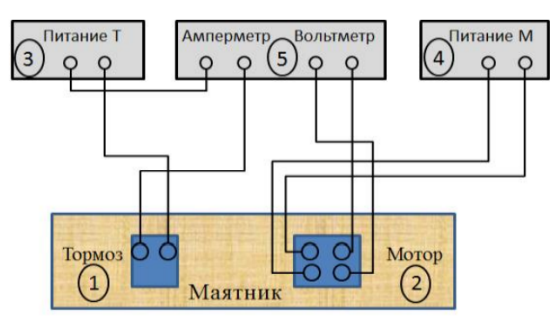
\includegraphics[width=0.9\textwidth]{img/scheme.png}
	\caption{Схема установки}
\end{figure}
